\documentclass{homework}
\usepackage{siunitx}
\newcommand{\hwname}{Zooey Nguyen}
\newcommand{\hwemail}{zooeyn@ucla.edu}
\newcommand{\hwclass}{Astro 81}
\newcommand{\hwtype}{Homework}
\newcommand{\hwnum}{1}

\begin{document}
\maketitle

\question
\begin{alphaparts}
    \questionpart Mass of the black hole in grams.
    \begin{align*}
        m	&= 	4 \vdot \num{e6} \vdot  M_\odot  \\
            &=  \num{4e6} \vdot \SI{1.989e30}{\kilogram}    \\
            &=  \SI{7.956e36}{\kilogram} \vdot \frac{\SI{1000}{\gram}}{\SI{1}{\kilogram}}   \\
            &=  \boxed{\SI{7.956e39}{\gram}}
    \end{align*}
    \questionpart Distance to the black hole in meters, then lightyears.
    \begin{align*}
        d   &=  \SI{8}{kpc} \vdot \frac{\SI{1000}{pc}}{\SI{1}{kpc}} \vdot \frac{\SI{3.08e16}{\metre}}{\SI{1}{pc}} \\
            &=  \boxed{\SI{2.448e20}{\metre}}    \\
            &=  \SI{8}{kpc} \vdot \frac{\SI{1000}{pc}}{\SI{1}{kpc}} \vdot \frac{\SI{3.26}{ly}}{\SI{1}{pc}}  \\
            &=  \boxed{\SI{26080}{ly}}
    \end{align*}
    \questionpart Same as the number of lightyears away, \fbox{26080 years} ago. According to a Google search this was in the Stone Age when humans were primarily hunter-gatherers.
\end{alphaparts}

\question
Using the relation $R = r\theta$ where $R$ is the radius of the object, $r$ is the distance to the object, and $\theta$ is the angular radius of the object in radians. We want to find $\Theta_{moon}$ and $\Theta_\odot$, the Diameters of the Moon and the Sun. First the angular diameter of the Moon:
\begin{align*}
    \Theta_{moon}	&=  2\theta_{moon} \\
                    &=  \frac{2 R_{moon}}{r_{moon}} \\
                    &=  \frac{2 \SI{1.7371e6}{\metre}}{\SI{384.4e6}{\metre}} \vdot \frac{\SI{360}{\degree}}{\SI{2\pi}{\radian}} \\
                    &=  \boxed{\SI{0.5178}{\degree}}    \\
                    &=  \SI{0.5178}{\degree} \vdot  \frac{3600''}{\SI{1}{\degree}}  \\
                    &=  \boxed{1864''}
\end{align*}
Then the angular diameter of the Sun:
\begin{align*}
    \Theta_{moon}	&=  2\theta_{moon} \\
                    &=  \frac{2 R_{moon}}{r_{moon}} \\
                    &=  \frac{2 \SI{696.34e6}{\metre}}{\SI{149.6e9}{\metre}} \vdot \frac{\SI{360}{\degree}}{\SI{2\pi}{\radian}} \\
                    &=  \boxed{\SI{0.5333}{\degree}}    \\
                    &=  \SI{0.5333}{\degree} \vdot  \frac{3600''}{\SI{1}{\degree}}  \\
                    &=  \boxed{1920''}
\end{align*}

\question
I have a coffee rarely since my body cannot handle caffeine and likely never will, so let's say yearly around 10, and the human lifespan is on the scale of around 100 years, so I'll estimate I'll have probably \fbox{1000 coffees} in my lifetime. This seems reasonable: I don't think I'll have so few as to have only around 100 coffees in total since I used to drink more often, but I'm certainly not drinking around 100 coffees a year since I drink it much more rarely than a couple times a week.

\question
I live in Los Altos, CA. The latitude is \fbox{\SI{37.38}{\degree}} and the longitude is \fbox{\SI{122.11}{\degree}} west. I Googled it but I also remember the latitude by heart because I think at some point there was a group of high-schoolers here that created a band called 37 Degrees.

\question
On January 20, 2021, it will have been exactly 10 months since the vernal equinox, when the Sun's right ascension is 0h. Since the right ascension shifts by a full 24h every 12 months, it shifts by 2h per month. Thus the right ascension of the Sun on inauguration day is $\SI{10}{month} \vdot \frac{\SI{2}{\hour}}{\SI{1}{month}} = \boxed{\SI{20}{\hour}}$.

\question
Since the mean solar time is the hour angle of the Sun plus 12 hours, the mean solar time difference is just the difference between the local hour angles of the Sun between London and Sydney, or the difference in angle it takes for the Sun to culminate above Sydney and then above London. The Sun culminates on the meridian, meaning the difference in culmination angle between two points on Earth is simply the difference in longitude between them. Also, 24 hours in mean solar time corresponds to 360 degrees around the globe, which is the range that longitude measures. Thus the difference in mean solar time between London and Sydney is $(\SI{151}{\degree} E - \SI{0}{\degree} E) * \frac{\SI{24}{\hour}}{\SI{360}{\degree}} = \boxed{\SI{10}{\hour}}$.

\question
The hour angle of an object is 0h, and equivalently 24h, when it crosses the meridian. If Rigel is at 20h for a particular observer, it has just \fbox{4h} more to go till it transits the meridian.

\question
I need to record my \fbox{latitude, longitude, and time} in the day I observed it at that particular altitude and azimuth. The relative position of the object in the sky to me will vary as an arc over the entire day. The apparent trajectory of the arc is dependent on my position on Earth, meaning the altitude and azimuth will vary together on an arc throughout the day. The object's point on the trajectory, corresponding to the exact altitude and azimuth I observe, is dependent on the time of day.

\question
We have $a_{min} = \SI{20}{\degree}$ and $a_{max} = \SI{70}{\degree}$, where the star is South of the zenith. We can first get the declination from these two values.
\begin{align*}
    \var	&= 	\frac{1}{2} (a_{max} + a_{min})\\
            &=  \frac{1}{2} (\SI{90}{\degree})  \\
            &=  \boxed{\SI{45}{\degree}}
\end{align*}

We can then use the corresponding equation for maximum altitude when the star's peak transit crosses South of the zenith.
\begin{align*}
    a_{max}	&= 	\SI{90}{\degree} - \varphi + \var   \\
    \SI{70}{\degree}    &=  \SI{90}{\degree} - \varphi + \SI{45}{\degree}   \\
    \varphi &=  \boxed{\SI{65}{\degree}}
\end{align*}

\question
\begin{alphaparts}
    \questionpart Use the relation in the textbook for $a_{max}$ and $a_{min}$.
    \begin{align*}
        a_{max}	&= 	\SI{90}{\degree} - (\varphi - \var) \\
                &=  \SI{90}{\degree} - (\SI{20}{\degree} - \SI{-29}{\degree}) \\
                &=  \SI{90}{\degree} - \SI{49}{\degree} \\
                &=  \boxed{\SI{41}{\degree}}    \\
        a_{min} &=  (\varphi + \var) - \SI{90}{\degree} \\
                &=  (\SI{20}{\degree} + \SI{-29}{\degree}) - \SI{90}{\degree} \\
                &=  \SI{-99}{\degree}   \\
                &=  \boxed{\SI{-81}{\degree}}
    \end{align*}
    \newpage
    \questionpart Drawing of celestial sphere as observed by Keck.
    \begin{figure}[htbp]
        \centering
        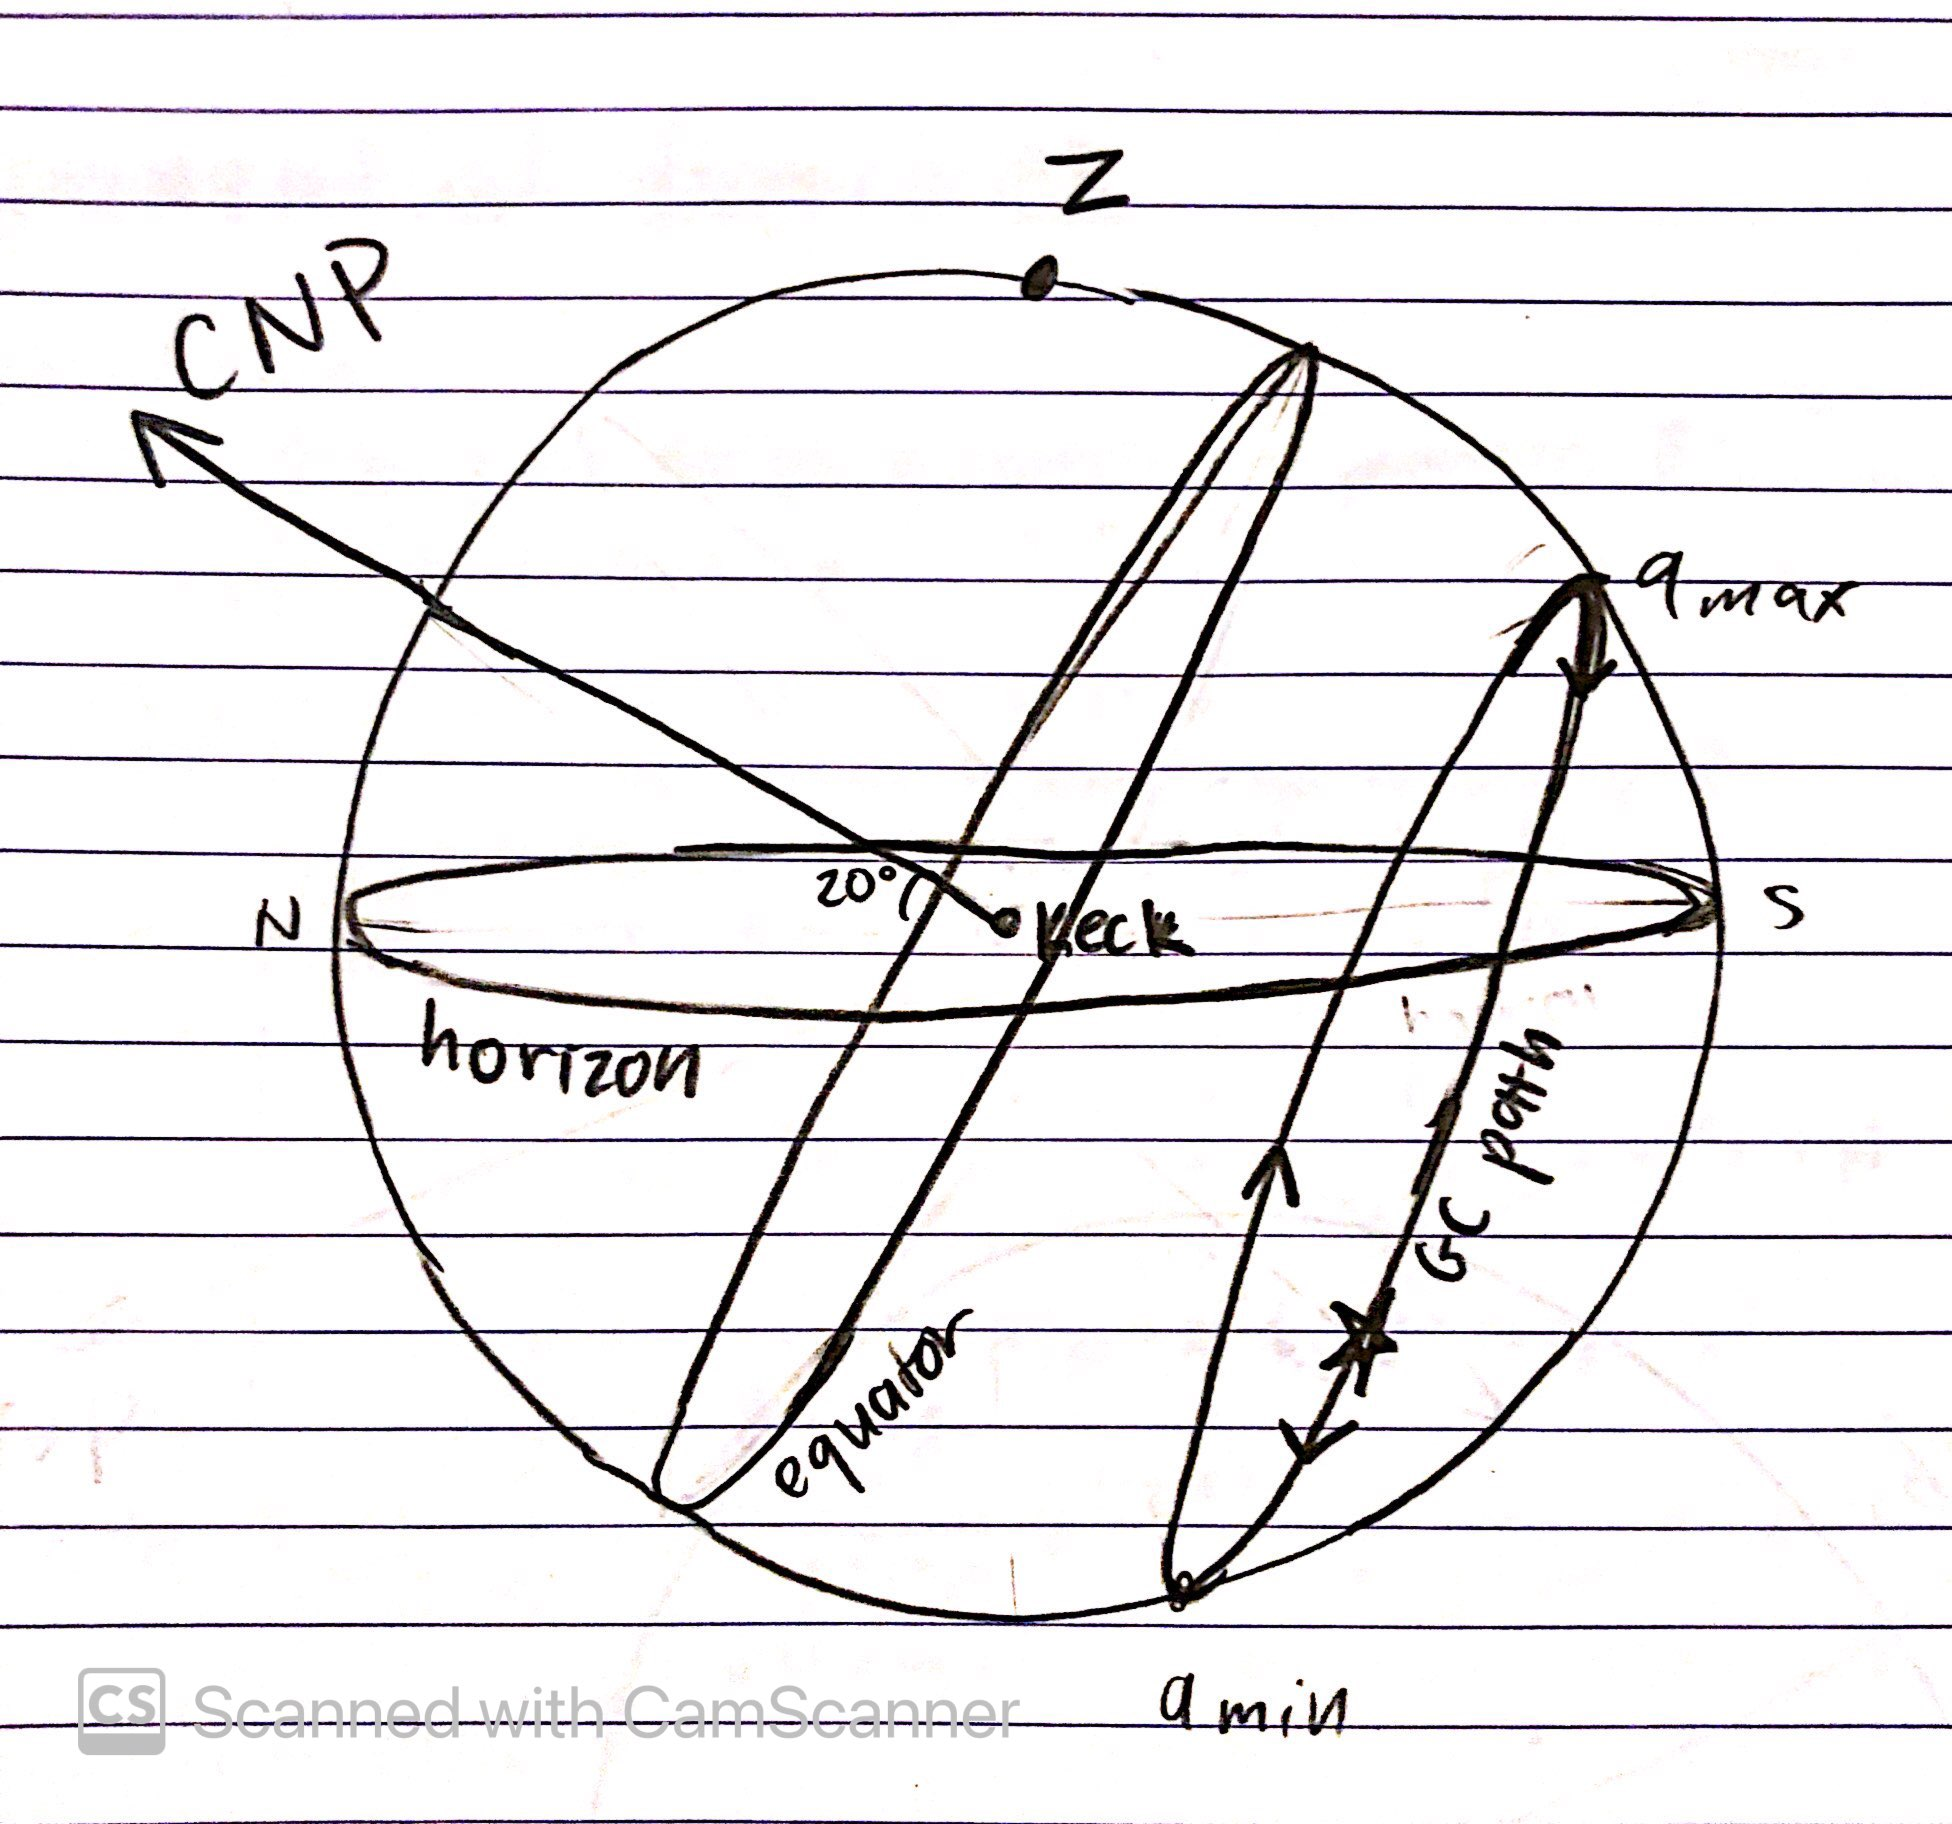
\includegraphics[width=0.7\linewidth]{gc_keck.jpg}
    \end{figure}
    
    \questionpart We are considering it being circumpolar about the South Pole so let's temporarily switch to positive numbers for easier reference, as if we're considering an object at $\var = \SI{29}{\degree}$ being circumpolar about the North Pole. Then the latitudes for which it is circumpolar is defined:
    \begin{align*}
        \var    &>  \SI{90}{\degree} - \varphi  \\
        \varphi &>  \SI{90}{\degree} - \var \\
        \varphi &>  \SI{90}{\degree} - \SI{29}{\degree} \\
        \varphi &>  \SI{61}{\degree}
    \end{align*}
    So if it were the case for a star with that positive declination, latitudes of \SI{61}{\degree} and more would see it as circumpolar. But we flipped this on its head so just invert. Latitudes of \fbox{\SI{-61}{\degree} and below} will see it as circumpolar.
    \questionpart Hawaii is where Keck is so we need to find the point where the hour angle of the Galactic center at Keck is 0h. Since $HA_{center} = LST - RA_{center}$, then $LST = RA_{center}$, thus the local sidereal time has to be 18h. The solar time, which we want to find, is the hour angle of the Sun. If the local sidereal time is 18h, then we have $HA_\odot = 18h - RA_\odot$. The hour angle of the Sun $HA_\odot$ is always defined as 0h, or equivalently, 24h. So we get that $RA_\odot = 6h$, which means that the Sun is 6 of 24 hours through its loop around the celestial sphere passing through the vernal equinox. This means the Sun is 6/24=1/4 through the year, or 3 months. Vernal equinox is on March 20, so three months after that, June 20, is the summer equinox. The Galactic center transits above Keck at midnight in the \fbox{summer}.
\end{alphaparts}

\question
For half the year the North Pole faces away from the Sun, and for the other half it faces towards the Sun. Any view of the Sun is entirely determined by Earth's orbit about the Sun because at the North Pole there's no difference in the relative position in space throughout the day. The Sun must rise and set only \fbox{once} a year.

\question
A solar day is \fbox{longer} than a sidereal day. If the Earth rotated in the opposite direction the solar day would be shorter by the same amount since a given point on Earth would hit the line towards the Sun a bit earlier than in a full sidereal rotation. If its rotational speed were twice as fast, the sidereal day and the solar day would both be half-time, so the difference would also be half the time, and opposite in sign to the actual difference $\Delta t$. So the time difference would become \boxed{-\frac{1}{2} \Delta t}.

\end{document}
